\section{Einleitung}
	\label{sec:einleitung}
	Dieser Versuch behandelt ged"ampfte und erzwungende Schwingungen am Beispiel des LC-Kreises.
	Schaltet man eine Induktivit"at mit einer Kapazit"at in Reihe, k"onnen sie ihre Energie periodisch austauschen (Abb \ref{fig:lc-kreis}).
	Durch einen Ohmschen Wiederstand im Schaltkreis geht bei jedem Zyklus energie in Form von W"arme verloren und die Schwingung wird ged"ampft.
	Schlie"slich l"asst sich eine Schwingung anregen, indem man eine "au"sere, periodische Spannung anlegt.
	Hierbei treten verschiedene Resonanzph"anomene auf.
	
	\begin{figure}[h!]
		\centering
		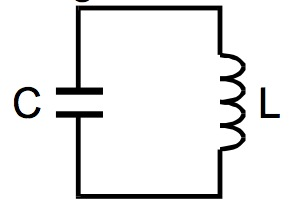
\includegraphics[width = 15cm]{img/lc-kreis.jpg}
		\caption{Ein LC-Kreis: Energie, die im System vorhanden ist, wird periodisch zwischen Kondensator und Spule ausgetauscht.}
		\label{fig:lc-kreis}
	\end{figure}

\section{Theorie}
	\label{sec:theorie}
